\chapter{FPGA: historical introduction, structure, design flow, VHDL and use in the MoVe\_IT project}
\section{Introduction}
\noindent Digital electronics is concerned with circuits which represent information using a finite set of output
states. Most of the applications use in fact just two states, which are often labelled ‘0’ and ‘1’.
Behind this choice is the fact that the whole Boolean formalism then becomes available for the
solution of logic problems, and also that arithmetic using binary representations of numbers is a very
mature field\cite{fpga1}.
\newline
In addition, having only two
different values for the voltages or currents used to represent states is the safest choice in terms of
design margins in order to protect the data from the noise.



\section{Programmable Logic Devices history}
\noindent Historically, TTL (Transistor–Transistor Logic) chips fuelled an initial wave of digital system designs in
the 1970s.
%This section will focus on the separate branches that evolved to satisfy the demand
%for programmability of different logic functions.
By programmability, it is meant the ability of a
designer to affect the logic behaviour of a chip after it has been produced in the factory.
\newline
\noindent A first improvement in the direction of programmability came with the introduction of gate
arrays, which were nothing else than a chip filled with NAND gates that the designer could
interconnect as needed to generate any logic function he desired.
This interconnection had to happen
at the chip design stage, thus before production, but it was already a convenient improvement over
designing everything from scratch. Until the introduction of Programmable Logic
Arrays (PLAs) in the 1980s no real programmable solution was available. These were two-level AND-OR
structures with user-programmable connections.
%\begin{figure}[H]
%	\centering
%	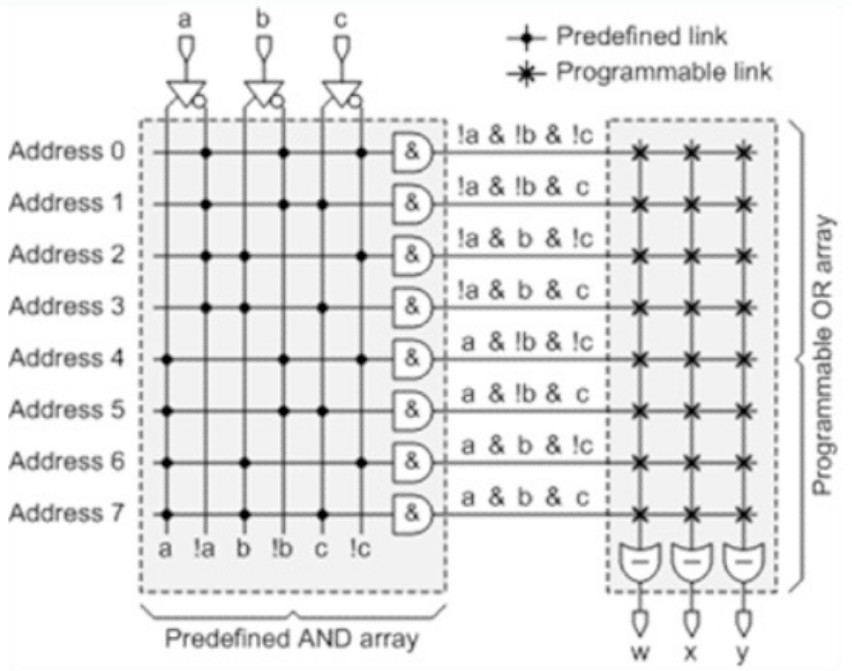
\includegraphics[width=0.7\linewidth]{IMG/ch3/PLD}
%	\caption{Unprogrammed PROM (Fixed AND Array, Programmable OR Array)}
%	\label{fig:pld}
%\end{figure}

\noindent Programmable Array Logic (PAL) devices were an
improvement in performance and cost over the PLA structure. Today, these devices are collectively
called Programmable Logic Devices (PLDs).

\noindent The next stage in sophistication resulted in Complex PLDs (CPLDs), which were nothing else
than a collection of multiple PLDs with programmable interconnections. FPGAs, in turn, contain a
much larger number of simpler blocks with the attendant increase in interconnect logic, which in fact
dominates the entire chip.
\begin{figure}[H]
	\centering
	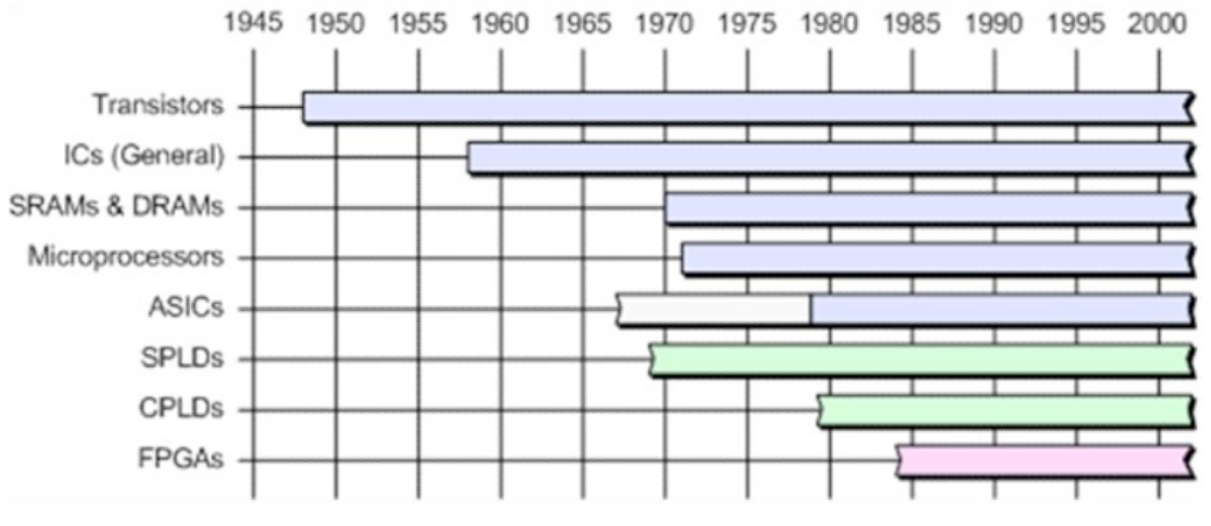
\includegraphics[width=0.7\linewidth]{IMG/ch3/TIME}
	\caption{Appearance over the years of programmable logic devices\cite{fpga3}}
	\label{fig:time}
\end{figure}
%\subsection{FPGA}
\noindent Xilinx introduced the first Field Programmable Gate Arrays
(FPGAs) in 1984, though they were not called FPGAs until
Actel popularized the term around 1988\cite{fpga2}. Since their introduction, FPGA devices have progressed
through several distinct phases of development.
Each phase was driven by both process technology opportunity
and application demand. These driving pressures
caused observable changes in the device characteristics
and tools. Each age is eight years long and each
became apparent only in retrospect. The three ages are:
\begin{itemize}
	\item Age of Invention 1984–1991
	\newline
	The first FPGA, the Xilinx XC2064, contained only 64 logic blocks, each of which held two three-input Look-Up Tables (LUTs) and one register, less than 1000 gates.
	\item Age of Expansion 1992–1999
	%\newline
	
	\item Age of Accumulation 2000–2007
	%\newline
	
\end{itemize}

\section{FPGA Versus PAL}
\noindent Programmable logic was well established before the
FPGA. EPROM-programmed Programmable Array Logic
(PAL) had carved out a market niche in the early 1980s.
However, FPGAs had an architectural advantage. To understand
the FPGA advantage, we first look at the simple
programmable logic structures of these early 1980s devices.
A PAL device, as depicted in figure \ref{fig:pal}, consists of a two level
logic structure. Inputs are shown entering at
the bottom. On the left side, a programmable and array
generates product terms, ands of any combination of the
inputs and their inverses. A fixed or gate in the block at
the right completes the combinational logic function of the
macrocell’s product terms. Every macrocell output is an
output of the chip.
\begin{figure}[H]
	\centering
	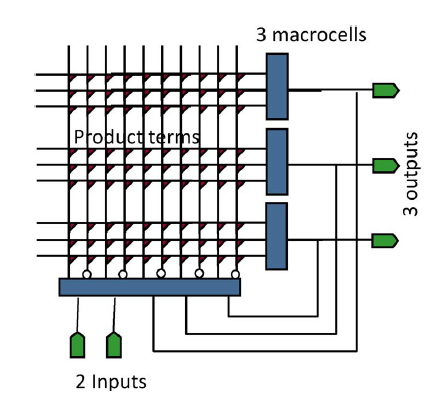
\includegraphics[width=0.7\linewidth]{IMG/ch3/PAL}
	\caption{Generic PAL architecture}
	\label{fig:pal}
\end{figure}
\noindent Nearly all common functions could be implemented in one pass through the PAL's macrocell array.
The delay through the PAL array is the same regardless of the function performed or where it is located in the array.
PALs had simple fitting software that mapped logic quickly to arbitrary locations in the array with no performance concerns.
PALs were very efficient from a manufacturing point of view.
However, the architectural issue with PALs is evident when one considers scaling. The number of programmable points in
the and array grows with the square of the number of inputs. PAL input and product-term lines are also
heavily loaded, so delay grows rapidly as size increases. To maintain speed, power consumption rose dramatically. Large PALs were
impractical in both area and performance.
\newline
The FPGA innovation was the elimination of the and array that provided the programmability. Instead, configuration
memory cells were distributed around the array to control functionality and wiring. This change gave up the
memory-array-like efficiency of the PAL structure in favor of architectural scalability. The architecture of the FPGA,
shown in figure 4, consists of an array of programmable logic blocks and interconnect with field-programmable switches.
\begin{figure}[H]
	\centering
	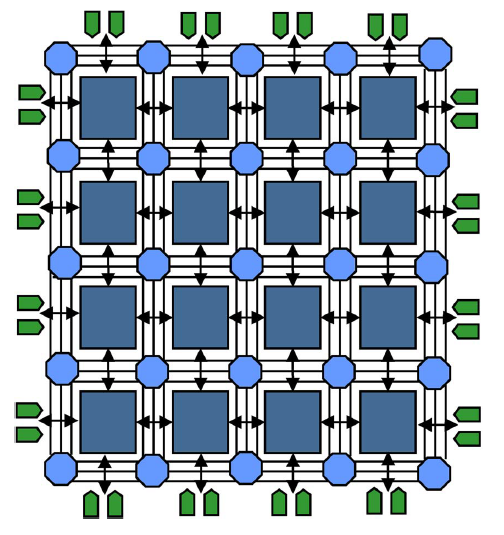
\includegraphics[width=0.7\linewidth]{IMG/ch3/FPGA}
	\caption{Generic array FPGA architecture. 4x4 array with three wiring
		tracks per row and column. Switches are at the circles at intersections.
		Device inputs and outputs are distributed around the array.}
	\label{fig:fpga}
\end{figure}
\noindent The consequences of this change were:
\begin{itemize}
	\item FPGA architecture could look nothing like a memory. Design and manufacturing were very different than memory.
	\item The logic blocks were smaller. There was no guarantee that a single function would fit into one. Therefore, it was difficult to determine ahead of time how much logic would fit into the FPGA.
	\item The performance of the FPGA depended on where the logic was placed in the FPGA. FPGAs required placement and routing, so the performance of the finished design was not easy to predict in advance.
	\item Complex EDA (Electronic Design Automation) software was required to fit a design into an FPGA.
\end{itemize}




\section{FPGA vs ASIC}
\noindent In the 1980s, Application-Specific Integrated Circuit
(ASIC) companies brought an amazing product to the
electronics market: the built-to-order custom integrated
circuit. By the mid-1980s, dozens of companies were selling
ASICs, and in the fierce competition, the winning attributes
were low cost, high capacity and high speed.When
FPGAs appeared, they compared poorly on all of these
measures, yet they thrived. The ASIC functionality was determined by custom mask
tooling. ASIC customers paid for those masks!
Because they had no custom tooling, FPGAs reduced the up-front
cost and risk of building custom digital logic. By making
one custom silicon device that could be used by hundreds or
thousands of customers, the FPGA vendor effectively
amortized the costs over all customers.
\begin{figure}[H]
	\centering
	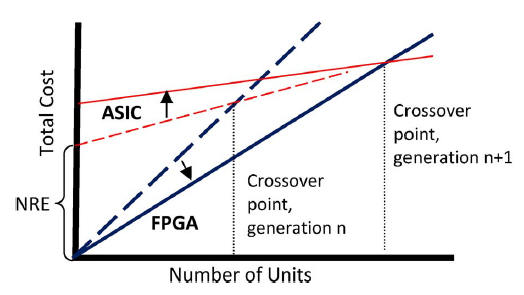
\includegraphics[width=0.7\linewidth]{IMG/ch3/COST}
	\caption{FPGA versus ASIC Crossover Point. Graph shows total cost
		versus number of units. FPGA lines are darker and start at the lower
		left corner. With the adoption of the next process node (arrows
		from the earlier node in dashed lines to later node in solid lines),
		the crossover point, indicated by the vertical dotted line, grew larger.
	\newline NRE (non-recurring engineering cost).}
	\label{fig:cost}
\end{figure}     
\noindent  An FPGA has no NRE charge, but each unit costs more than the
functionally equivalent ASIC, hence the steeper line. The
two lines meet at the crossover point. If fewer than that
number of units is required, the FPGA solution is cheaper;
more than that number of units indicates the ASIC has
lower overall cost.
\newline
Today, device cost is less of a driver in the FPGA
versus ASIC decision than performance, time-to-market,
power consumption, I/O capacity and other capabilities. Many ASIC customers use older process technology,
lowering their NRE cost, but reducing the per-chip cost
advantage. Not only did FPGAs eliminate the up-front masking
charges and reduce inventory costs, but they also reduced
design costs by eliminating whole classes of design problems.
These design problems included transistor-level design,
testing, signal integrity, crosstalk, I/O design and
clock distribution.

\section{FPGA structure}
\begin{figure}[H]
	\centering
	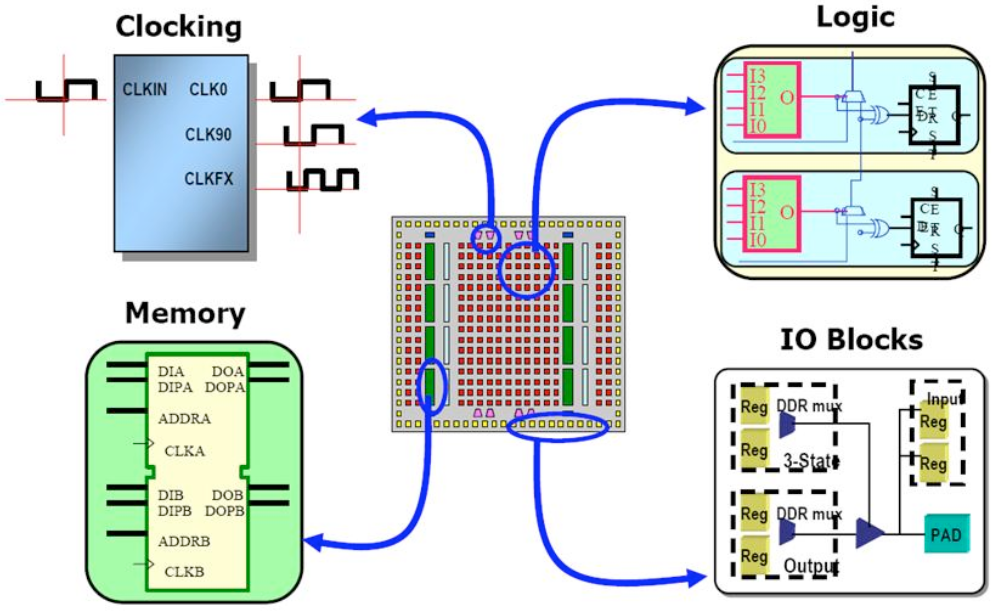
\includegraphics[width=0.7\linewidth]{IMG/ch3/FPGA2}
	\caption{Internal structure of a generic FPGA}
	\label{fig:fpga2}
\end{figure}
\noindent A typical modern FPGA, like in figure \ref{fig:fpga2}, provides the user with programmable logic blocks that
contain the pool of combinatorial blocks and flip-flops to be used in the design. In addition, vendors
acknowledge the fact that logic is often used with memory, and typically include
variable amounts of static Random Access Memory (RAM) inside their chips. Clock conditioning has
also become commonplace, and support in the form of Delay Locked Loops (DLLs) and Phase Locked
Loops (PLLs) is also provided inside the same silicon chip. Finally, an FPGA chip needs to be easily interfaced to other chips or
external signals. In order to make this interfacing easier, FPGA vendors have invested a great deal of
effort in enhancing the flexibility of the input/output blocks behind the chip pads. Each pad can serve
as an input, an output, or both. The list of electrical standards supported is extensive, and novel
techniques for maximizing bandwidth, such as clocking data in using both edges of the clock, are
widely supported.
\newline
All the components shown in figure \ref{fig:fpga2}, however, typically account for less than 20\% of the silicon
inside an FPGA chip. What is not shown is the large amounts of programmable interconnect and the
auxiliary circuits which ‘program’ the generic blocks to become a well-defined piece of logic.
To overcome the silicon inefficiency problem, FPGA vendors often include hardwired
Intellectual Property (IP) cores inside the chips for functions identified as recurrent in many designs.
These non-programmable blocks include general-purpose processors, high-speed serial interfaces,
arithmetic blocks and Ethernet Medium Access Control (MAC) units.
\\
FPGAs are truly parallel in nature so different processing operations do not have to compete for the same resources. As a result, the performance of one part of the application is not affected when additional processing is added.
\newline
\noindent In figure \ref{fig:fpga} it can be seen that the three more important blocks that made a FPGA chip are: Configurable logic Blocks (CBLs, blue squares); Input/Output Blocks (IOBs, green rectangles); Programmable Switch Matrixs (PSMs, blue octagon).
\begin{itemize}
	\item \textbf{CBLs}: Each CLB consists of n-input Lookup table and a pair of programmable flip flops. In Xilinx logic block, figure \ref{fig:clb}, a Look up table is used to implement any number of different functionality. The output of the lookup table gives the result of the logic function that it implements. Lookup table is implemented using SRAM (Static Random Access Memory).
	\begin{figure}[H]
		\centering
		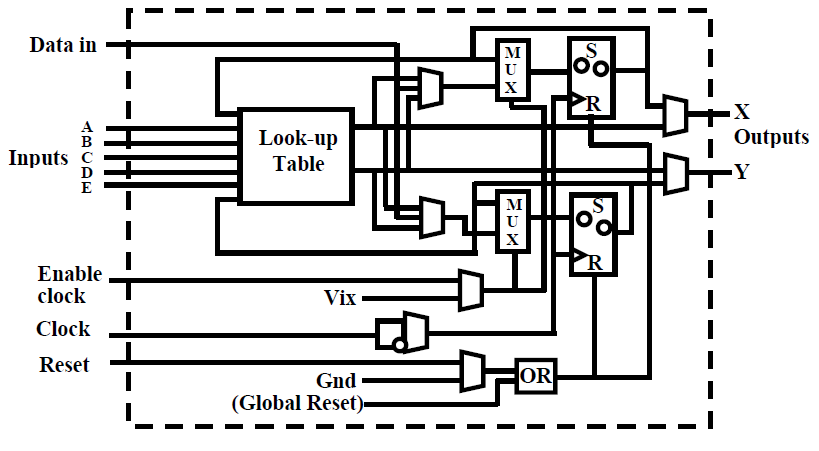
\includegraphics[width=0.7\linewidth]{IMG/ch3/CLB}
		\caption{Xilinx - LUT based configurable logic block}
		\label{fig:clb}
	\end{figure}
	\item \textbf{IOBs}: I/O blocks control functions such as tri-state buffer control, output transition speed (Slew Rate).
	\newline
	Provides to the chip a minimum of over-current and over-voltage protection and the right termination for each specific type of signalling.
	\item \textbf{PSMs}: Interconnects provide routing path. Using 6 CMOS switches controlled by a 6-bit data can be controlled a  wire intersection. Being \textbf{A}, \textbf{B}, \textbf{C} and \textbf{D} the  end of the routing the following connections can be made: \textbf{AB}, \textbf{AC}, \textbf{AD}, \textbf{BC}, \textbf{BD} and \textbf{CD}.
	\newline
	The data for each PSM is stored in a SRAM.
\end{itemize}
\noindent Thus a board its configured in two ways:
\begin{itemize}
	\item By setting the intersections (SMBs) between the logic blocks.
	\item By setting the function of each logic block.
\end{itemize}
\section{FPGA design flow and tools}
\noindent The most common flow nowadays used in the design of FPGAs involves the following
subsequent phases:
\begin{itemize}
	\item \textbf{Design entry}: This step consists in transforming the design ideas into some form of
	computerized representation. This is most commonly accomplished using Hardware Description
	Languages (HDLs). The two most popular HDLs are Verilog and the Very High Speed
	Integrated Circuit HDL (VHDL), used fot my thesis work. It should be noted that an HDL, as its name implies, is only
	a tool to describe a design that pre-existed in the mind, notes, and sketches of a designer. Another point to note is that HDLs differ from
	conventional software programming languages in the sense that they don’t support the concept
	of sequential execution of statements in the code. This is easy to understand if one considers the
	alternative schematic representation of an HDL file: what one sees in the upper part of the
	schematic cannot be said to happen before or after what one sees in the lower part.
	This is the only human-labour intensive part of the design process.
	\item \textbf{Simulation}: Typically, the design entry step is followed or interspersed with periods of functional simulation. That's where a simulator is used to execute the design and confirm that the correct outputs are produced for a given set of test inputs\cite{fpga4}. This section will be analyzed in more detail later on in this chapter.
	\item \textbf{Synthesis}: The synthesis tool receives HDL and a choice of FPGA vendor and model. From
	these two pieces of information, it generates a netlist which uses the primitives proposed by the
	vendor in order to satisfy the logic behaviour specified in the HDL files.
	\item \textbf{Place and route}: The placer takes the synthesized netlist and chooses a place for each of the
	primitives inside the chip. The router’s task is then to interconnect all these primitives together
	satisfying the timing constraints. The most obvious constraint for a design is the frequency of
	the system clock, but there are more involved constraints one can impose on a design using the
	software packages supported by the vendors.
	\item \textbf{Bit stream generation (Download)}: FPGAs are typically configured at power-up time from some sort of
	external permanent storage device, typically a flash memory. Once the place and route process is
	finished, the resulting choices for the configuration of each programmable element in the FPGA
	chip, be it logic or interconnect, must be stored in a file to program the flash.
	
\end{itemize}

\begin{figure}[H]
	\centering
	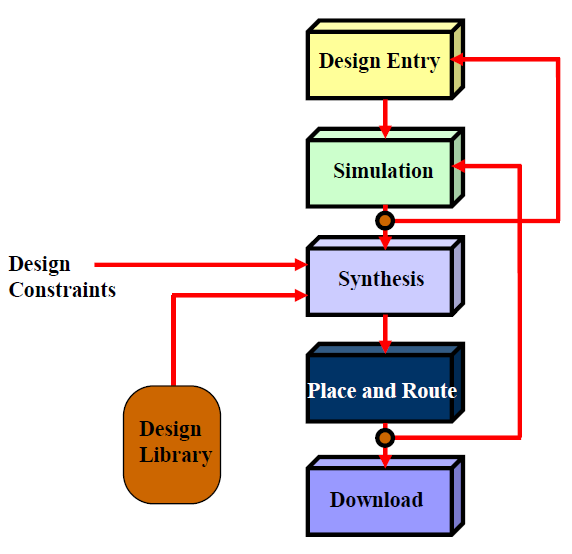
\includegraphics[width=0.7\linewidth]{IMG/ch3/FLOW}
	\caption{Programmable logic, in this case FPGA, design process}
	\label{fig:flow}
\end{figure}

\section{Hardware Description Language}
\begin{figure}[H]
	\centering
	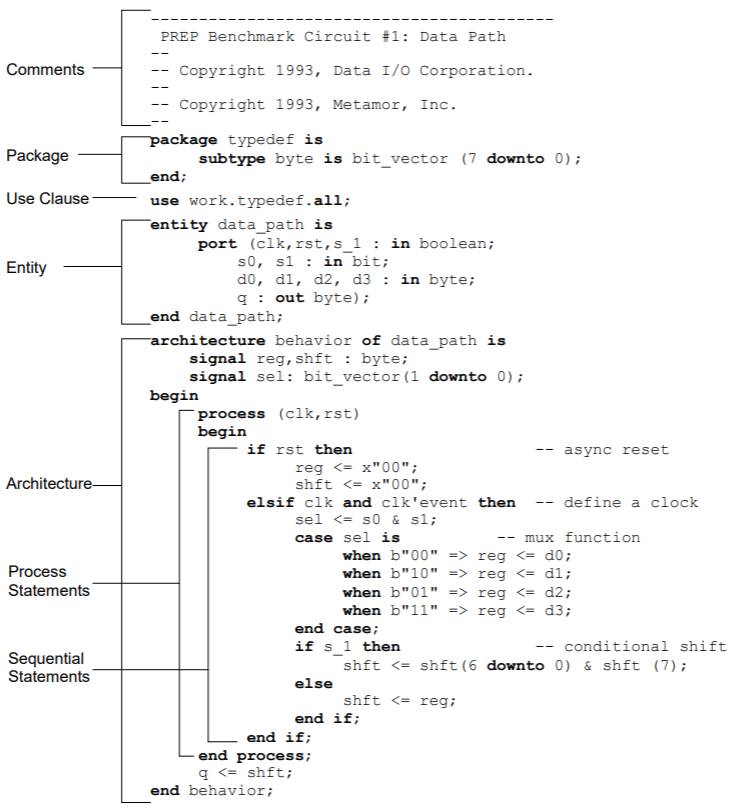
\includegraphics[width=0.7\linewidth]{IMG/ch3/VHDL}
	\caption{The structure of a VHDL design description}
	\label{fig:vhdl}
\end{figure}

\subsection{Entity}

\subsection{Architecture}

\subsection{Process}

\subsection{Constraints}


\section{Development tools}

\subsection{Vivado}

\subsection{LabView}

\section{Kintex 7 kc705}

































